\documentclass[a4paper,12pt]{article} 



%Добавляет возможность искать и копировать текст
\usepackage{cmap}

%Убирает пробел между названием таблицы/рисунка и самой таблицей/рисунком
\usepackage{caption}
\captionsetup[table]{skip= -0 cm}
\captionsetup[figure]{skip= -0 cm}

%Выравнивание названия таблиц по левому краю
%\usepackage[nooneline]{caption} 
%Размеры отступов 
\usepackage[left=20mm, top=20mm, right=20mm, bottom=20mm, footskip=10mm]{geometry}

%Рисунки
\usepackage{graphicx}
\usepackage{wrapfig} %обтекание элементов
\graphicspath{{graphs}{figures}}  % папки с картинками

%Русский язык в формулах
\usepackage{mathtext}

%  Русский язык
\usepackage[T2A]{fontenc}			
\usepackage[utf8]{inputenc}			
\usepackage[english,russian]{babel}	

%Готические буквы
\usepackage{amssymb}

% Математика
\usepackage{amsmath,amsfonts,amssymb,amsthm,mathtools} 
\usepackage{wasysym}

%Цветные подписи в таблице
\usepackage[table,xcdraw]{xcolor}

\usepackage{fancyhdr} % Колонтитулы
 	\pagestyle{fancy}
 	\renewcommand{\headrulewidth}{0.3mm}  % Толщина линейки, отчеркивающей верхний колонтитул
 	%\lfoot{Нижний левый}
 	%\rfoot{Нижний правый}
 	\rhead{Белостоцкий Артмемий, Б04-006}
 	%\chead{Верхний в центре}
 	\lhead{Лабораторная работа №4.2.1}
 	% \cfoot{Нижний в центре} % По умолчанию здесь номер страницы
 	
 	
\begin{document} 

%Титульник 
\begin{titlepage}
	\begin{center}
		\large 	МИНИСТЕРСТВО ОБРАЗОВАНИЯ И НАУКИ РОССИЙСКОЙ ФЕДЕРАЦИИ\\
				МОСКОВСКИЙ ФИЗИКО-ТЕХНИЧЕСКИЙ ИНСТИТУТ \\
				(НАЦИОНАЛЬНЫЙ ИССЛЕДОВАТЕЛЬСКИЙ ИНСТИТУТ)\\ 
				ФИЗТЕХ-ШКОЛА ЭЛЕКТРОНИКИ, ФОТОНИКИ \\
				И МОЛЕКУЛЯРНОЙ ФИЗИКИ \\
		
		
		\vspace{4.0 cm}
		Лабораторная работа № 4.2.1 \\ 
		\LARGE \textbf{Кольца Ньютона}
	\end{center}
	\vspace{3 cm} \large
	
	\begin{flushright}
		выполнил студент 2 курса \\
		{группы Б04-006}\\
		\textbf{Белостоцкий Артемий}\\
	\end{flushright}
	
	\vfill

	\begin{center}
	Долгопрудный, 2021 г.
	\end{center}
\end{titlepage}                                                                      

\section*{Цель работы}

Познакомиться с явлением интерференции в тонких пленках на примере колец Ньютона и с методикой интерфереционных измерений кривизны стеклянной поверхности.


\section*{В работе используются}
\begin{itemize}
\item измерительный микроскоп с опак-иллюминатором
\item плоско-выпуклая линза
\item пластинка из черного стекла 
\item ртутная лампа типа ДРШ
\item щель
\item линзы
\item призма прямого зрения
\item объектная шкала


\end{itemize}





\section*{Теоретическое введение}
	
	\begin{wrapfigure}{l}{0.35\linewidth} 
		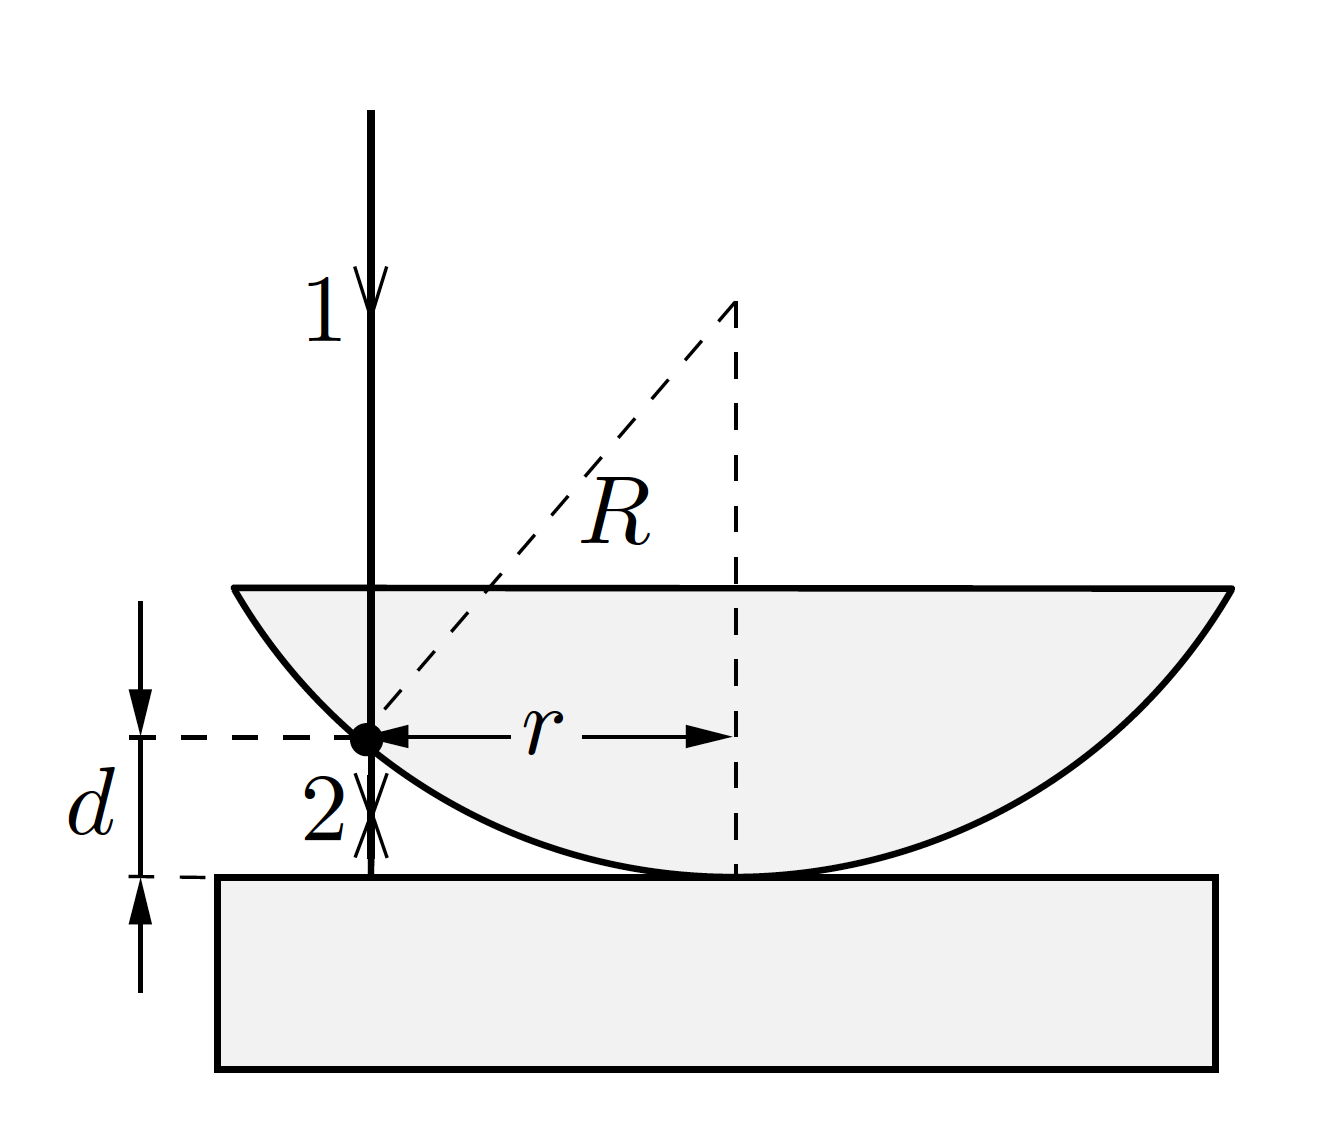
\includegraphics[width=\linewidth]{fig2}
		\caption{Экспериментальная установка}
		\label{ring}
	\end{wrapfigure}

	Этот классический опыт используется для определения радиуса кривизны сферических поверхностей линз. В этом опыте наблюдается интерференция волн, отражённых от границ тонкой воздушной прослойки, образованной сферической поверхностью линзы и плоской стеклянной пластиной. При нормальном падении света (рис. \ref{ring}) интерференционные полосы локализованы на сферической поверхности и являются полосами равной толщины.
	
	Геометрическая разность хода между интерферирующими лучами равна удвоенной толщине воздушного зазора $ 2d $ в данном месте. Для точки на сферической поверхности, находящейся на расстоянии $ r $ от оси системы, имеем $ r^2 = R^2 - (R - d)^2 = 2Rd - d^2 $, где $ R $ --- радиус кривизны сферической поверхности (рис. \ref{ring}).
	
	При $ R \gg d $ получим$  d = r^2/2R $. С учётом изменения фазы на $ \pi $ при отражении волны от оптически более плотной среды (на границе воздух-стекло) получим \textbf{оптическую разность хода интерферирующих лучей}:
	
	\begin{equation}\label{r_m}
	\Delta = \dfrac{\lambda}{2} + 2d = \dfrac{r^2}{2R} + \dfrac{\lambda}{2}
	\end{equation}
	
	Из условия интерференционного минимума $ \Delta = \dfrac{(2m +1)\lambda}{2}, \; m =0, 1, 2.. $ получим радиусы темных колец $ r_m $, а из аналогичного условия максимума $ \Delta = m \lambda $ радиусы светлых $ r_m' $ :
	
	\begin{equation}\label{r_m'}
	r_m = \sqrt{m \lambda R}, \qquad 	r_m' = \sqrt{\dfrac{(2m-1) \lambda R}{2}}
	\end{equation}
	
\newpage

\section*{Экспериментальная установка}

Схема экспериментальной установки приведена на рис. \ref{lab}. Опыт выполняется с помощью измерительного микроскопа.
На столик микроскопа помещается держатель с полированной пластинкой из
чёрного стекла. На пластинке лежит исследуемая линза.


	\begin{wrapfigure}{r}{0.5\linewidth} 
	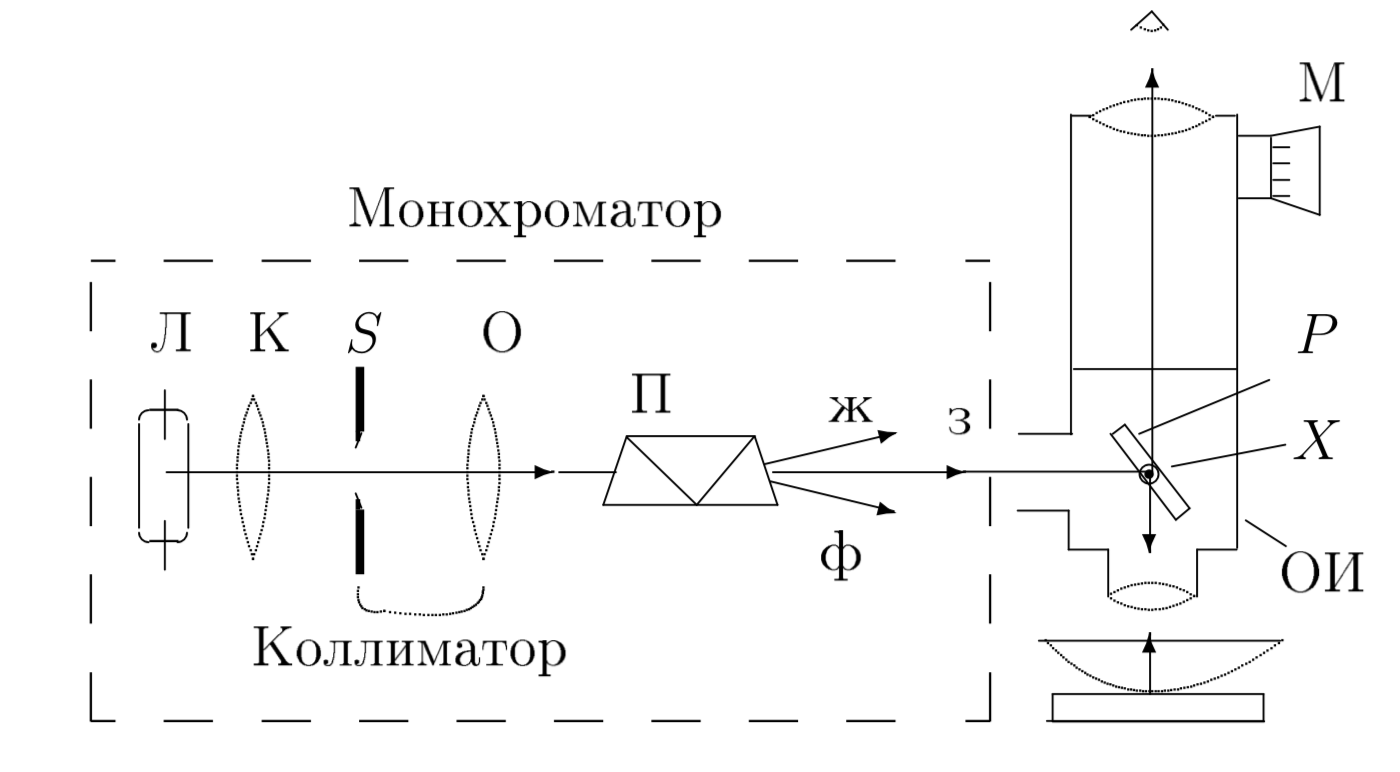
\includegraphics[width=\linewidth]{fig1}
	\caption{Экспериментальная установка}
	\label{lab}
\end{wrapfigure}

Источником света служит ртутная лампа, находящаяся в защитном кожухе. Для получения монохроматического света применяется призменный монохроматор, состоящий из конденсора $ К $, коллиматора (щель $ S $ и объектив $ О $) и призмы прямого зрения $ П $. Эти устройства с помощью рейтеров располагаются на оптической скамье. Свет от монохроматора попадает на расположенный между объективом и окуляром микроскопа опак-иллюминатор (ОИ)  специальное устройство, служащее для освещения объекта при работе в отражённом свете. Внутри опак-иллюминатора находится полупрозрачная стеклянная пластинка P, наклоненная под углом $ 45^\circ $ к оптической оси микроскопа. Свет частично отражается от этой пластинки, проходит через объектив микроскопа и попадает на исследуемый объект. Пластинка может поворачиваться вокруг горизонтальной оси $ X $, опак-иллюминатор вокруг вертикальной оси.

	Столик микроскопа может перемещаться в двух взаимно перпендикулярных направлениях помощью винтов препаратоводителя. Отсчетный крест окулярной шкалы перемещается перпендикулярно оптической оси с помощью микрометрического винта $ М $.
	
	Оптическая схема монохроматора позволяет получить в плоскости входного окна опак-иллюминатора достаточно хорошо разделённые линии спектра ртутной лампы. Изображение щели $ S $ фокусируется на поверхность линзы объективом микроскопа, т.е. точка источника и точка наблюдения спектра совпадают.Интерференционная картина не зависит от показателя преломления линзы и определяется величиной зазора между линзой и пластинкой (кольца равной толщины).

	Сначала микроскоп настраивается на кольца Ньютона в белом свете (свете ртутной лампы), затем при помощи монохроматора выделить из спектра яркую зелёную линию и провести измерения диаметров колец в монохроматическом свете. 


\newpage

\section*{Ход работы}
\subsubsection*{Измерение диаметров колец}
Включим ртутную лампу и настроим микроскоп на кольца Ньютона в зеленом свете. ($\lambda = 546 нм$). Перемещая перекрестие, будем последовательно устанавливать его на середины темных и светлых колец и записывать соответствующие показание окуляра. Учтем, что для начального положения перекрестия $-$ $r_0 = 6,92 \ дел $. Полученные данные занесем в Таблицу 1:

\begin{table}[h]
\begin{center}
\caption{}
\begin{tabular}{|c|c|c|c|c|}
\hline
 $r_m$, дел & m & $r_m'$, дел & 2m - 1 \\ \hline 
 0,12      & 1 & 0,32       & 1      \\ \hline
 0,51      & 2 & 0,75       & 3      \\ \hline
 1,06      & 3 & 1,18       & 5      \\ \hline
 1,35      & 4 & 1,47       & 7      \\ \hline
 1,59      & 5 & 1,71       & 9      \\ \hline
 1,86      & 6 & 1,97       & 11     \\ \hline
\end{tabular}
\end{center}
\end{table} 

Учитывая систематическую погрешность микроскопа $\sigma_{r_m} = \sigma_{r'_m}  = 0,01 \  дел$, построим график зависимости $r^2(f(m))$. Где

$$
f(m) = \begin{cases}
2m - 1, \text{ для светлых колец } \\
m, \text{ для темных колец }
\end{cases}
$$ 

$$
r^2 =  \begin{cases}
2r_m'^2, \text{ для светлых колец } \\
r_m^2, \text{ для темных колец }
\end{cases}
$$

\begin{figure}[h!]
	\begin{center}
	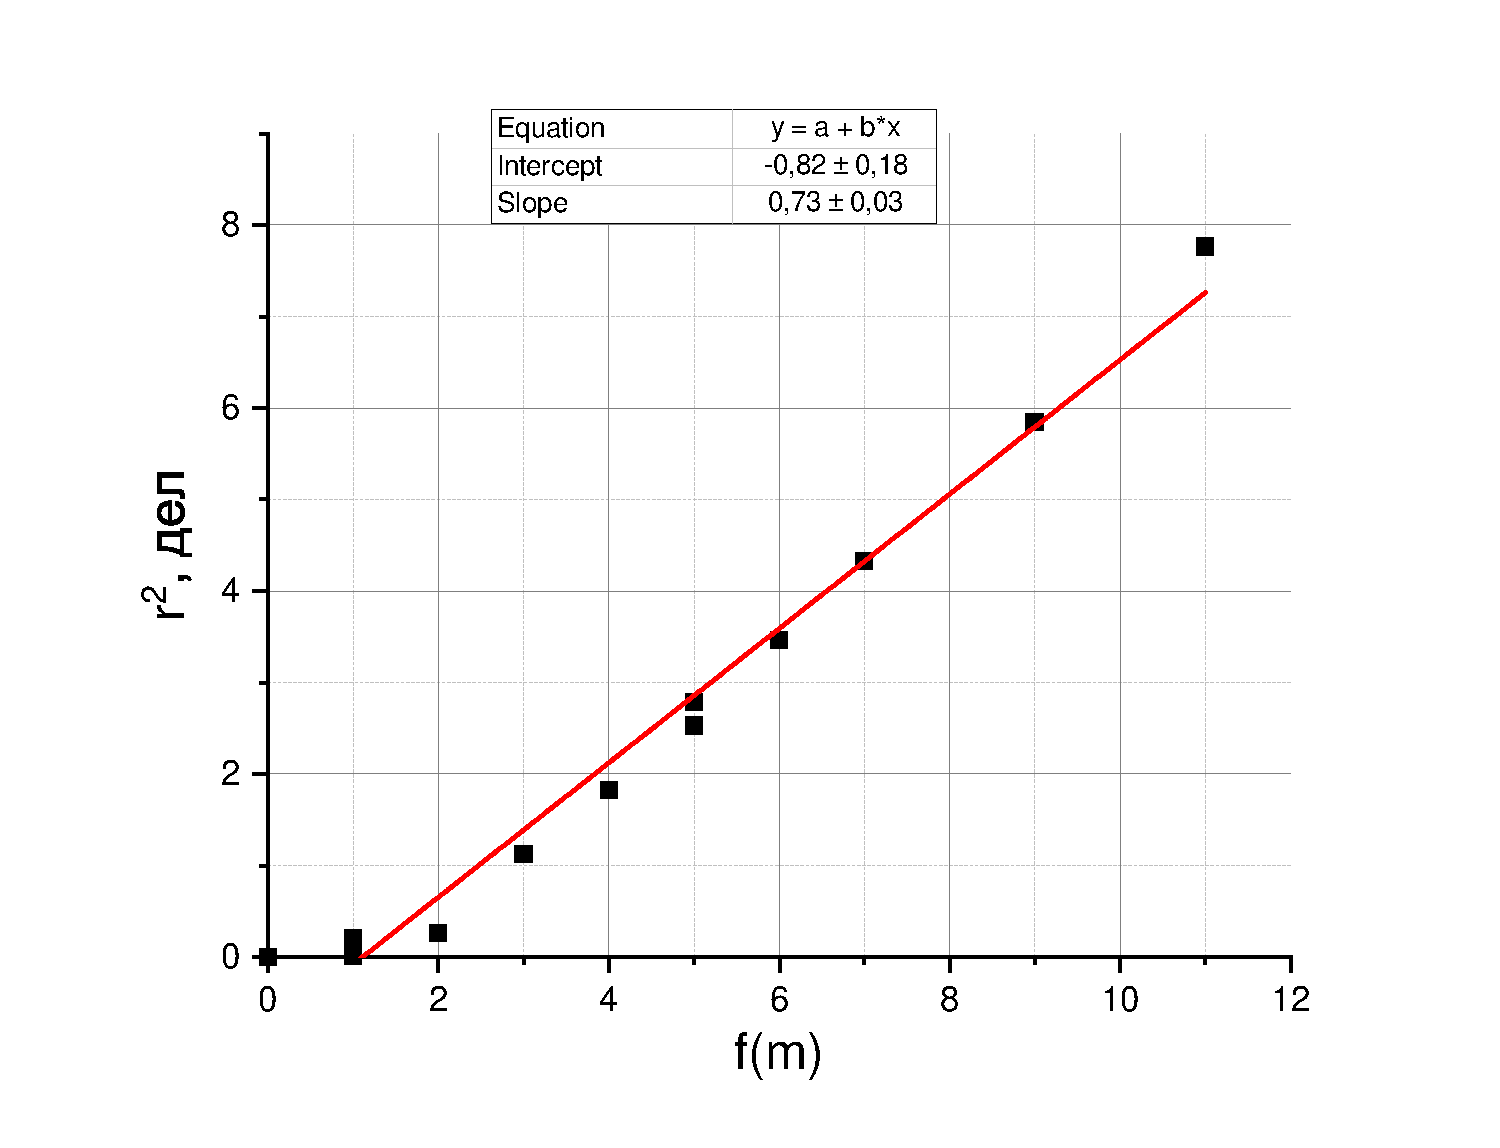
\includegraphics[scale=0.49]{graph1}
	\label{fig:setup}
	\caption{Зависимость $r^2(f(m))$}
	\end{center}
\end{figure}

\newpage

По МНК найдем коэффициент наклона графика:

$$
k = \lambda R \approx 0,73 \pm 0,03 \ дел^2
$$

Зная длину волну зеленой линии Hg: $ \lambda_{з} = 546 \ нм $ и цену деления микроскопа $\alpha = 0,1 \frac{мм}{дел}$ рассчитаем радиус кривизны линзы R:

$$
R = \frac{k \alpha^2}{\lambda_{з}} \approx 1,34 \ см
$$

$$
\sigma_{R} = R \frac{\sigma_{k}}{k} \approx 0,05 \ см 
$$

Окончательно: 

$$
R = 1,34 \pm 0,05 \ см
$$

\subsubsection*{Наблюдение <<Биений>>}

Осветим входное окно опак-иллюминатора сразу двумя спектральными компонентами ртути (желтой и зеленой).Получим картину биений и просчитаем количество темных полос от центра одной четкой системы полос до центра соседней четкой системы $-$ $\Delta m = 16$. Отсюда находим

$$
\Delta \lambda = \frac{\lambda_{з}}{\Delta m} \approx 34 \ нм
$$

\section*{Выводы}

1.В результате работы был получен радиус кривизны линзы $ R = 1,34 \pm 0,05 \ см$
\\
2.Также, была оценена разность длин волн желтой и зеленой спектральных компонент Hg $\Delta \lambda \approx 34 \ нм$, которая хорошо соотносится с теоретическим значением $\Delta \lambda = 33 \ нм$






\end{document}